\documentclass{article} % Define o tipo de documento
\usepackage{tikz}
\usepackage{array} % Necessário para o formato p{}
\usepackage{graphicx} % Se decidir usar o \resizebox mais tarde
\usetikzlibrary{positioning} 

% Sua macro \n{...} deve ser mantida:
\newcommand{\n}[1]{%
    \begin{tikzpicture}[scale=0.35, baseline=(current bounding box.center), every node/.style={circle,draw,minimum size=2mm,inner sep=1pt,font=\tiny}]
        \node {#1};
    \end{tikzpicture}%
}
% ...

\begin{document} % O corpo do documento começa aqui

\section*{Tabela de Exemplo} % Opcional, para dar um título

% Use a versão simplificada para o teste de sintaxe
\begin{center}
    \begin{tabular}{|p{4cm}|c|p{2cm}|} 
    \hline 
    \textbf{Fila (Queue)} & \textbf{Saída} & \textbf{Ação} \\
    \hline
    % Linha 1: Árvore Inicial (Encapsulada)
    \parbox[c]{4cm}{\centering % <-- NOVO: Força o TikZ a ser tratado como um bloco
        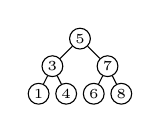
\begin{tikzpicture}[
            scale=0.35, baseline=(current bounding box.center),
            level distance=10mm, level 1/.style={sibling distance=20mm}, level 2/.style={sibling distance=10mm},
            every node/.style={circle,draw,minimum size=2mm,inner sep=1pt,font=\tiny}
        ]
          \node {5} child {node {3} child {node {1}} child {node {4}}} child {node {7} child {node {6}} child {node {8}}};
        \end{tikzpicture}
    }
    & {[]} & Inicia \\
    \hline

    % Linha 2: Fila com Árvores Parciais (Encapsulada)
    \parbox[c]{4cm}{\centering
        \begin{tikzpicture}[baseline=(current bounding box.center), node distance=5mm] 
            \node (A) at (0,0) {
                \begin{tikzpicture}[scale=0.35,level distance=10mm,sibling distance=10mm,every node/.style={circle,draw,minimum size=2mm,inner sep=1pt,font=\tiny}]
                    \node {3} child {node {1}} child {node {4}};
                \end{tikzpicture}
            };
            \node (B) [right=of A] {
                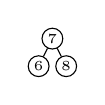
\begin{tikzpicture}[scale=0.35,level distance=10mm,sibling distance=10mm,every node/.style={circle,draw,minimum size=2mm,inner sep=1pt,font=\tiny}]
                    \node {7} child {node {6}} child {node {8}};
                \end{tikzpicture}
            };
        \end{tikzpicture}
    }
    & {[}5{]} & Processa 5 \\
    \hline

    % Linha 3 (e seguintes): Usando \n{...} (Encapsulada)
    \parbox[c]{4cm}{\centering
        \begin{tikzpicture}[baseline=(current bounding box.center), node distance=5mm]
            \node (A) at (0,0) {
                \begin{tikzpicture}[scale=0.35,level distance=10mm,sibling distance=10mm,every node/.style={circle,draw,minimum size=2mm,inner sep=1pt,font=\tiny}]
                    \node {7} child {node {6}} child {node {8}};
                \end{tikzpicture}
            };
            \node (B) [right=of A] {\n{1}}; 
            \node (C) [right=of B] {\n{4}}; 
        \end{tikzpicture}
    }
    & {[}5,3{]} & Processa 3 \\
    \hline
    
    % Linha 4: Fila de Nós Simples
    \parbox[c]{4cm}{\centering
        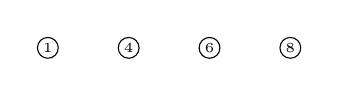
\begin{tikzpicture}[baseline=(current bounding box.center), node distance=5mm]
            \node (A) at (0,0) {\n{1}}; 
            \node (B) [right=of A] {\n{4}}; 
            \node (C) [right=of B] {\n{6}}; 
            \node (D) [right=of C] {\n{8}}; 
        \end{tikzpicture}
    }
    & {[}5,3,7{]} & Processa 7 \\
    \hline

    % Linha 5
    \parbox[c]{4cm}{\centering
        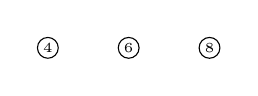
\begin{tikzpicture}[baseline=(current bounding box.center), node distance=5mm]
            \node (A) at (0,0) {\n{4}};
            \node (B) [right=of A] {\n{6}};
            \node (C) [right=of B] {\n{8}};
        \end{tikzpicture}
    }
    & {[}5,3,7,1{]} & Processa 1 \\
    \hline

    % Linha 6
    \parbox[c]{4cm}{\centering
        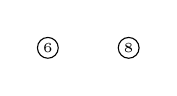
\begin{tikzpicture}[baseline=(current bounding box.center), node distance=5mm]
            \node (A) at (0,0) {\n{6}};
            \node (B) [right=of A] {\n{8}};
        \end{tikzpicture}
    }
    & {[}5,3,7,1,4{]} & Processa 4 \\
    \hline

    % Linha 7
    \parbox[c]{4cm}{\centering
        
\begin{tikzpicture}[baseline=(current bounding box.center), node distance=5mm]
            \node (A) at (0,0) {\n{8}};
        \end{tikzpicture}
    }
    & {[}5,3,7,1,4,6{]} & Processa 6 \\
    \hline

    % Linha 8
    {} & {[}5,3,7,1,4,6,8{]} & Termina \\
    \hline
    \end{tabular}
\end{center}

\end{document} % O documento termina aqui